\documentclass{article}
\usepackage{amsfonts}
\usepackage{graphicx}
\usepackage{enumitem}
\usepackage{amsmath}
\usepackage{float}
\usepackage{tfrupee}
\usepackage{gensymb}
\usepackage{romannum}
\begin{document}
\begin{enumerate}
\item If $x=3$ is one root of the quadratic equation $x^2-2kx-6=0$. Then find the value of $k$.
\item What is the $HCF$ of smallest prime number and the smallest composite number?
\item In an $AP$,if the common difference $(d)$=$-4$,and the seventh term $(a_{7})$ is 4, then find the first term.
\item Given that $\sqrt{2}$ is irrational, prove that $(5+\sqrt[3]{2})$ is an irrational number.
\item In $Fig.1$,$ABCD$ is a rectangle.Find the values of $x$ and $y$.
	\begin{figure}[H]
        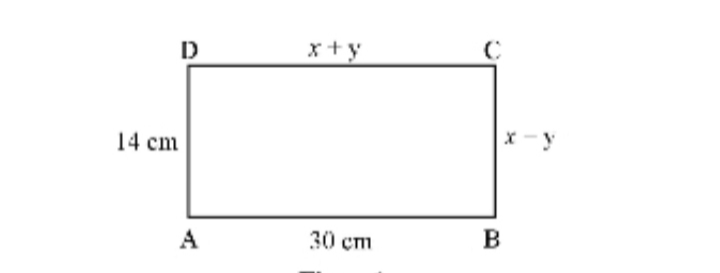
\includegraphics [width=\columnwidth] {./IMAGE3.jpg}
	\label{fig:fig1}
	\caption{rectangular ABCD}
	\end{figure}
\item Find the sum of first $8$ multiples of $3$.
\item A plane left $30 minutes$ late than its scheduled time and in order to reach the destination $1500km$ away in time, it had to increase its speed by $100km/h$ from the usual speed.Find its usual speed.
\item Prove that the area of an equilateral triangle discribed on one side of the square is equal to half the area of the equilateral triangle described on one of its diagonal.
\item If the area of two similar triangles are equal, prove that they are congruent.
\item Prove that the lengths of tangents drawn from an external point to a circle are equal.
\item A wooden article was made by scooping out a hemisphere from each end of a solid cylinder, as shown in $Fig.2$. If the height of the cylinder is $10cm$ and its base is of radius $3.5cm$. Find the total surface area of the article.
	\begin{figure}[H]
		\centering
		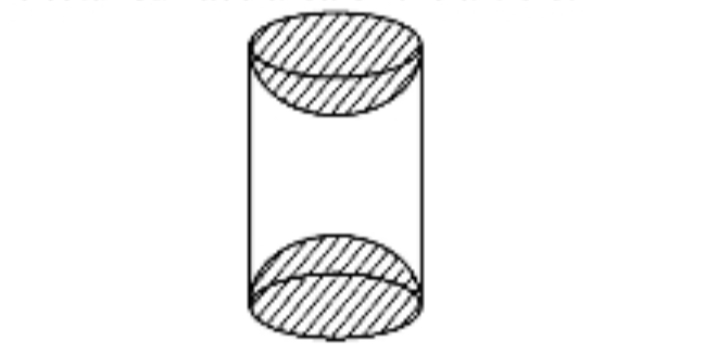
\includegraphics [width=\columnwidth] {./IMAGE2.jpg}
		\label{fig:fig2}
		\caption{cylinder}
	\end{figure}
\item A heap of rice is in the form of a cone of base diameter $24m$ and height $3.5m$. Find the volume of the rice. How much canvas cloth is required to just cover the heap?
\item The table below shows the salaries of $280$ persons \\
	\begin{tabular}{|c|c|} \\
		\hline
		(salary in thousand\rupee) & No. of persons\\ \hline
		$5-10$ & $49$\\ \hline
		$10-15$ & $133$\\ \hline
		$15-20$ & $63$\\ \hline
		$20-25$ & $15$\\ \hline
		$25-30$ & $6$\\ \hline
		$30-35$ & $7$\\ \hline
		$35-40$ & $4$\\ \hline
		$40-45$ & $2$\\ \hline
		$45-50$ & $1$\\ \hline
	\end{tabular} \\
		Calculate the median salary of the data.
\item Draw a triangle $ABC$ with $BC=6cm$, $AB=5cm$ and $\angle=60\degree$.Then constuct a triangle whose sides are $\frac{3}{4}$ of the corresponding sides of the $\Delta ABC$.
\item The sum of four consecutive numbers in an $AP$ is $32$ and the ratio of the product of the first and last term to the product of two middle terms is $7:15$. Find the numbers.
\item In an equilateral $\triangle ABC$, $D$ is a point on side $BC$ such that BD=$\frac{1}{3}$BC. Prove that $9(AD)^2=7(AB)^2$.
\item Prove that, in a right triangle, the square on the hypotenuse is equal to the sum of the squares on the other two sides.
\item A motor boat whose speed is $18km/hr$ in still water takes $1hr$ more to go $24km$ upstream than to return down stream to the same spot. Find the speed of the stream.
\item A train travels at a certain average speed for a distance of $63km$ and then travels at a distance of $72km$ at an average speed of $6km/hr$ more than its original speed. If it takes $3 hours$ to complete total journey, what is original average speed?
\end{enumerate}
\end{document}
